\small
\section{赝势理论(续)}       %Bookmark
\subsection{基态总能量表达式}
\frame
{
	\frametitle{晶体总能量的一般表示\footnote{本部分参阅文献\cite{XIE-LU,R.Martin}}}
采用赝势方法计算的晶体总能量$E_T$由晶格中的电子能量$E_{e-e}$与离子实排斥能$E_{N-N}$之和:
	\begin{displaymath}
		E_T=E_{e-e}+E_{N-N}=T[\rho]+E_{ext}+E_{\mathrm{Coul}}+E_{\mathrm{XC}}+E_{N-N}
	\end{displaymath}
根据\textrm{Kohn-Sham}方程,其中动能泛函用单电子能量表示为
\begin{displaymath}
	T[{\rho}]=\sum_in_i\langle\psi_i|\varepsilon_i-V_{\mathrm{KS}}|\psi_i\rangle
\end{displaymath}
$n_i$是$\psi_i$上的电子占据数,$\varepsilon_i$是其能量本征值,因此有
\begin{displaymath}
	\hspace*{-12.0pt}	E_T=\sum_in_i\varepsilon_i-\dfrac12\int\int\mathrm{d}\vec r\mathrm{d}\vec r\dfrac{\rho(\vec r)\rho(\vec r^{\prime})}{|\vec r-\vec r^{\prime}|}+\int\mathrm{d}\vec r\rho(\vec r)[\epsilon_{\mathrm{XC}}(\vec r)-V_{\mathrm{XC}}(\vec r)]+E_{N-N}
\end{displaymath}
}

\frame
{
	\frametitle{晶体总能量倒空间的表示}
周期体系的总能量表达式在动量空间($\vec K$空间)计算更方便
\begin{displaymath}
	\hspace*{-15.0pt}	E_T=\textcolor{red}{\sum_in_i\varepsilon_i}-\dfrac{\Omega}2\sum_{\textcolor{red}{\vec k\neq 0}}\rho^{\ast}(\vec k)V_{\mathrm{Coul}}(\vec k)+\Omega\sum_{\vec k}\rho^{\ast}(\vec k)[\epsilon_{\mathrm{XC}}(\vec k)-V_{\mathrm{XC}}(\vec k)]+E_{N-N}
\end{displaymath}
其中$V_{\mathrm{Coul}}(\vec k)$、$\epsilon_{\mathrm{XC}}(\vec k)$与$\rho^{\ast}(\vec k)$分别是\textrm{Coulomb}相互作用、单个电子的交换-相关能、交换-相关势和电子密度的\textrm{Fourier}分量。

由\textrm{Poisson}方程
\begin{displaymath}
	\nabla^2V_{\mathrm{Coul}}(\vec r)=-4\pi\rho(\vec r)
\end{displaymath}
的\textrm{Fourier}展开有
\begin{displaymath}
	V_{\mathrm{Coul}}(\vec k)=\dfrac{4\pi\rho^{\ast}(\vec k)}{|\vec k|^2}
\end{displaymath}
交换-相关势和交换-相关能的计算一般先在实空间计算$\epsilon_{\mathrm{XC}}(\vec r)$和$V_{\mathrm{XC}}(\vec r)$后,再通过\textrm{Fourier}变换到动量空间,得到$\epsilon_{\mathrm{XC}}(\vec k)$和$V_{\mathrm{XC}}(\vec k)$
}

\frame
{
	\frametitle{晶体离子相互作用的计算}
	离子间\textrm{Coulomb}相互作用能之和
	\begin{displaymath}
		E_{N-N}=\dfrac12\sum_{\vec R,s}\sideset{}{^{\prime}}\sum_{\vec R^{\prime},\vec s^{\prime}}\dfrac{Z_sZ_{s^{\prime}}}{|\vec R+\vec r_s-\vec R^{\prime}-\vec r_s^{\prime}|}
	\end{displaymath}
	这里$Z_s$是离子实的电荷数,$\vec R$表示晶格点的位矢,$\vec r_s$代表元胞内原子的相对位矢。

	\textcolor{red}{\textbf{注意}}:~$E_{N-N}$求和有无穷多项,\textcolor{red}{是发散的};~$V_{\mathrm{Coul}}(\vec k=0)$\textcolor{red}{是发散的}
	
	$V_{ext}$在不存在其他外场时,一般只考虑离子-电子的\textrm{Coulomb}相互作用,
	\begin{displaymath}
%		\begin{aligned}
			V_{ext}(\vec r)=\sum_{\vec R,s}\dfrac{-Z_s}{|\vec r-\vec R-\vec r_s|}\equiv\sum_{\vec R,s}v_{ext}^s(\vec r-\vec R-\vec r_s)
%		\end{aligned}
	\end{displaymath}
	$V_{ext}$的\textrm{Fourier}分量在$\vec k=0$\textcolor{red}{也是发散的}
}

\frame
{
	\frametitle{晶体总能量计算的奇点排除}
这三项单独都是发散的,但因为整个体系出于电中性,所以这些发散项相互抵消,是一个常数。因此求解\textrm{Kohn-Sham}方程时,先将$V_{\mathrm{Coul}}(\vec k=0)$和$V_{ext}(\vec k=0)$同时置为零,这相当于\textcolor{red}{将势能作一平移,或者说重新定义势能零点,而在总能量计算中补偿这一平移。}
\begin{figure}[h!]
	\begin{center}
		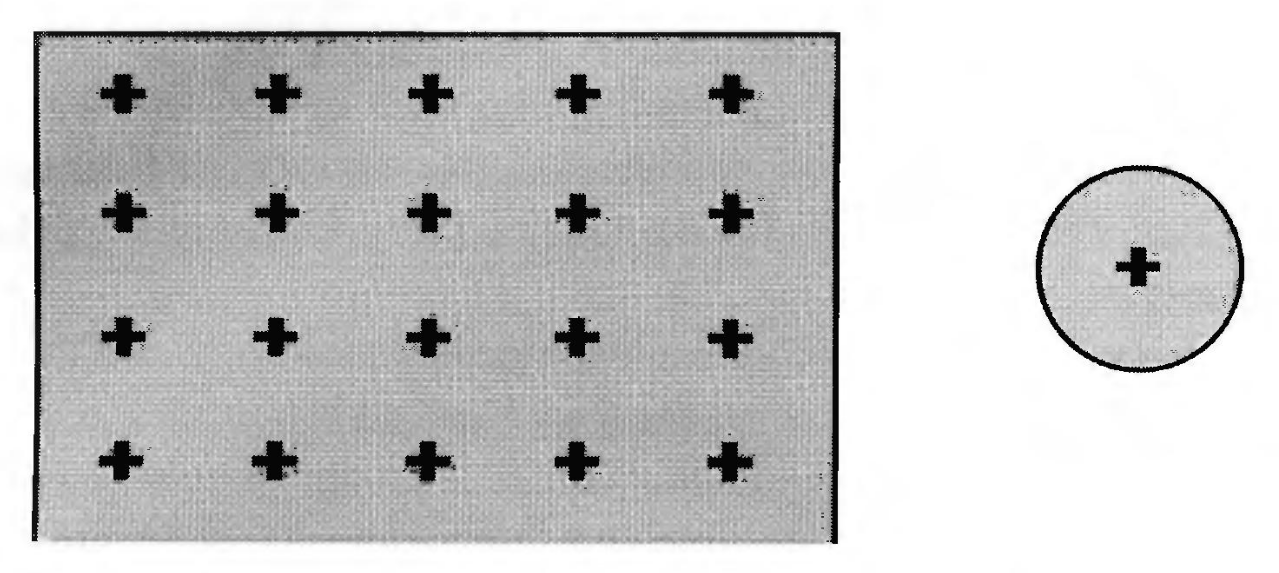
\includegraphics[height=0.65in,width=1.50in,viewport=0 0 1250 565,clip]{Figures/Ewald_method-3.png}
	\end{center}
	\caption{\fontsize{5.5pt}{2.2pt}\selectfont{\textrm{A lattice of point charge in a uniform compensating background as considered in the Ewald calculation.}}}
	\label{fig:Ewald-method-3}
\end{figure}
	发散项之和为:
	\begin{displaymath}
		\begin{aligned}
			\lim_{\vec k\rightarrow0}\Omega&\bigg[\dfrac12V_{\mathrm{Coul}}(\vec k)+\sum_sv_{ext}^s(\vec k)\bigg]\rho^{\ast}(\vec k)+\dfrac12\sum_{\vec R,s}\sideset{}{^{\prime}}\sum_{\vec R^{\prime},\vec s^{\prime}}\dfrac{Z_sZ_{s^{\prime}}}{|\vec R+\vec r_s-\vec R^{\prime}-\vec r_s^{\prime}|}\\
			=&\sum_s\alpha_s\sum_sZ_s+E_{\mathrm{Ewald}}
		\end{aligned}
	\end{displaymath}
}

\frame
{
	\frametitle{发散项的处理}
	对于形如$Z_s/r$的外场,其\textrm{Fourier}分量在$\vec k=0$附近展开
	\begin{displaymath}
		v_{ext}^s(\vec k)=-\dfrac{4\pi Z_s}{\Omega|\vec k|^2}+\alpha_s+O(\vec k); 
	\end{displaymath}
	展开$\rho^{\ast}(\vec k)$,有
	\begin{displaymath}
		\lim_{\vec k\rightarrow 0}\rho^{\ast}(\vec k)=\dfrac{\sum_sZ_s}{\Omega}+\beta|\vec k|^2+O(\vec k)
	\end{displaymath}
去掉高次项,有
\fontsize{8.5pt}{5.2pt}\selectfont{
\begin{displaymath}
	\begin{aligned}
		\lim_{\vec k\rightarrow 0}&\bigg[\boxed{\textcolor{blue}{\dfrac{\Omega}2\dfrac{4\pi[\rho^{\ast}(\vec k)]^2}{|\vec k|^2}}}+\boxed{\Omega}\bigg(\boxed{\textcolor{blue}{-\dfrac{4\pi\sum_sZ_s}{\Omega|\vec k|^2}}}+\sum_s\alpha_s\bigg)\boxed{\rho^{\ast}(\vec k)}+\boxed{\textcolor{red}{\dfrac12\dfrac{4\pi(\sum_sZ_s)^2}{\Omega|\vec k|^2}}}\bigg]\\
		&+\boxed{\dfrac12\sum_{\vec R,s}\sideset{}{^{\prime}}\sum_{\vec R^{\prime},\vec s^{\prime}}\dfrac{Z_sZ_{s^{\prime}}}{|\vec R+\vec r_s-\vec R^{\prime}-\vec r_{s^{\prime}}|}-\lim_{\vec k\rightarrow0}\textcolor{red}{\dfrac12\dfrac{4\pi(\sum_sZ_s)^2}{\Omega|\vec k|^2}}}\\
		=&\sum_s\alpha_s\sum_sZ_s+\textcolor{magenta}{E_{\mathrm{Ewald}}}
	\end{aligned}
\end{displaymath}}
}

\frame
{
	\frametitle{离子间相互作用的\textrm{Ewald}求和}
\begin{figure}[h!]
\centering
\vspace*{-0.20in}
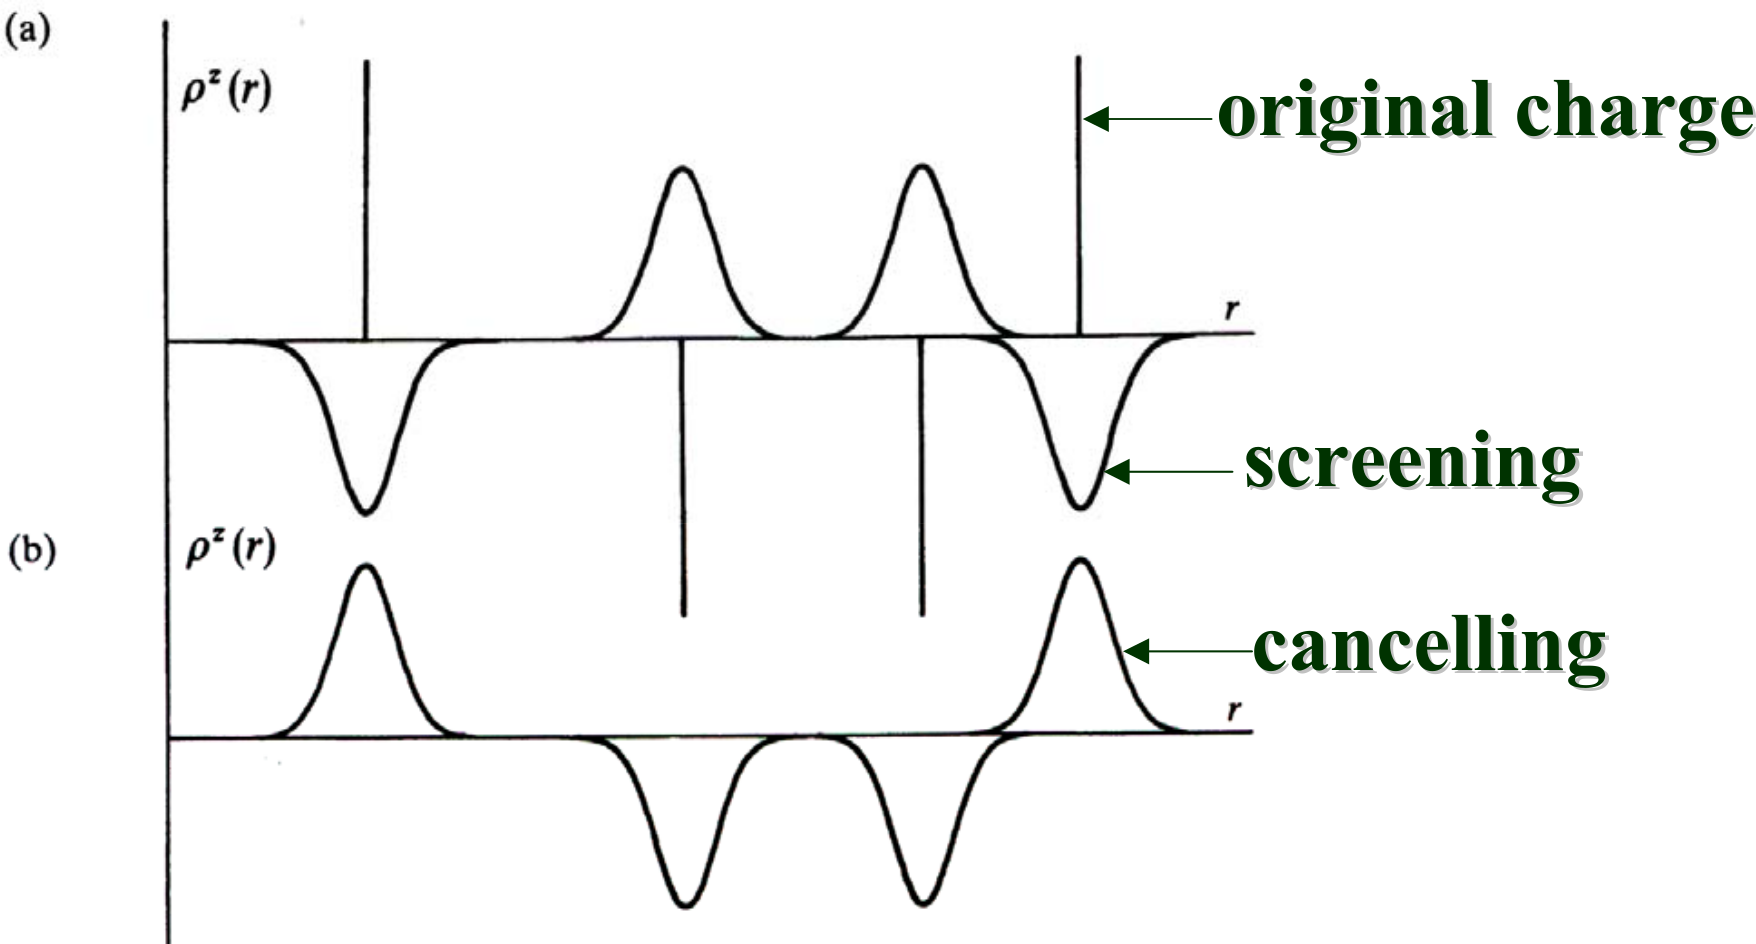
\includegraphics[height=2.3in,width=4.12in,viewport=0 0 1800 955,clip]{Figures/Ewald_method-2.png}
\caption{\fontsize{5.5pt}{2.2pt}\selectfont{\textrm{Each charge be screened by a Gaussian charge distribution of opposite sign and equal magnitude: $\rho_i(r)=\dfrac{Z_i\eta^3}{\pi^{3/2}}\mathrm{e}^{-\eta^2r^2}$.}}}%(与文献\cite{EPJB33-47_2003}图1对比)
\label{Ewald_method-2}
\end{figure}
}

\frame
{
	\frametitle{离子间相互作用的\textrm{Ewald}求和}
\begin{figure}[h!]
\centering
%\vspace*{-0.20in}
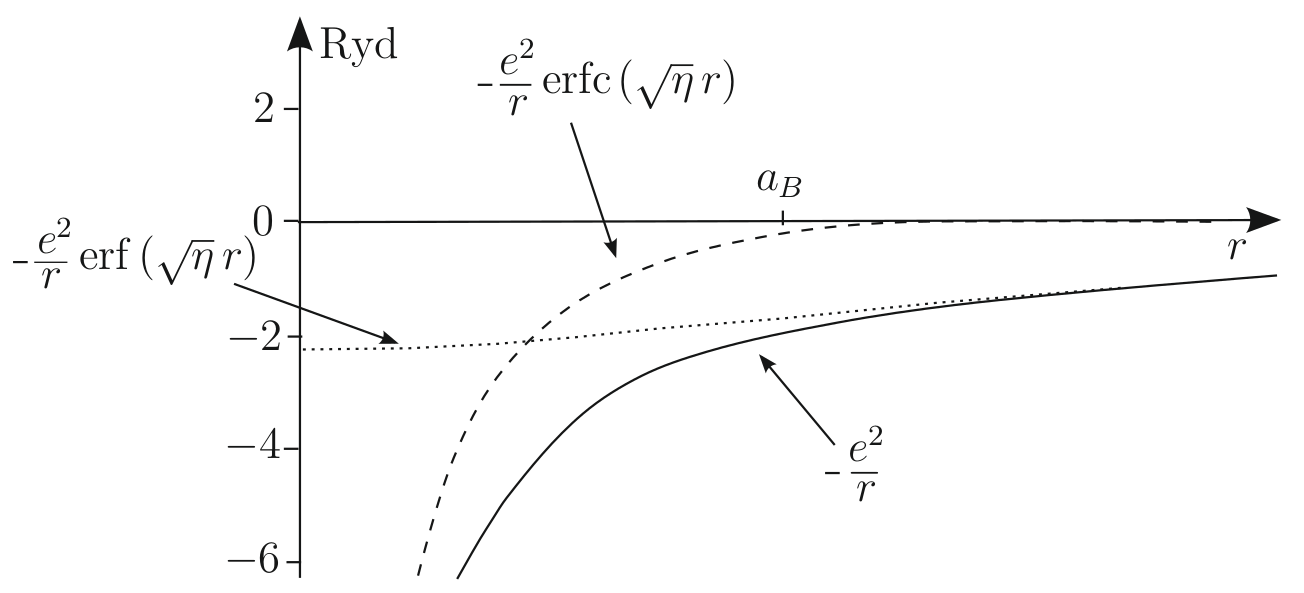
\includegraphics[height=1.8in,width=4.12in,viewport=0 0 1100 455,clip]{Figures/Ewald_method.png}
\caption{\fontsize{5.5pt}{2.2pt}\selectfont{\textrm{Decomposition of the potential $-e^2/r$ (singular at the origin and of long-range nature) into a contribution $-(e^2/r)\mathrm{erf}(\sqrt{\eta}r)$(regular at the origin of long-range) and a contribution $-(e^2/r)\mathrm{erfc}(\sqrt{\eta}r)$ (singular at the origin and of short-range nature). Here $\sqrt{\eta}=1 (\mathrm{Bohr radius unit})$ is chosen.}}}%(与文献\cite{EPJB33-47_2003}图1对比)
\label{Error_Function}
\end{figure}
}

\frame
{
	\frametitle{离子间相互作用的\textrm{Ewald}求和}
	\begin{displaymath}
		\begin{aligned}
			E_{\textrm{Ewald}}=&\dfrac12\sum_{\vec R,s}\sideset{}{^{\prime}}\sum_{\vec R^{\prime},\vec s^{\prime}}\dfrac{Z_sZ_{s^{\prime}}}{|\vec R+\vec r_s-\vec R^{\prime}-\vec r_{s^{\prime}}|}-\lim_{\vec k\rightarrow0}\dfrac12\times\dfrac{4\pi(\sum_sZ_s)^2}{\Omega|\vec k|^2}\\
			=&\dfrac12\sum_{\vec R,s}\sideset{}{^{\prime}}\sum_{\vec R^{\prime},\vec s^{\prime}}\dfrac{Z_sZ_{s^{\prime}}}{|\vec R+\vec r_s-\vec R^{\prime}-\vec r_{s^{\prime}}|}-\dfrac1{2\Omega}\sum_{s,s^{\prime}}\int\mathrm{d}\vec r\dfrac{Z_sZ_{s^{\prime}}}r\\
			=&\sum_{s,s^{\prime}}Z_sZ_{s^{\prime}}\bigg\{\dfrac{2\pi}{\Omega}\sum_{\vec k\neq 0}\cos[\vec k\cdot(\vec r_s-\vec r_{s^{\prime}})]\dfrac{\mathrm{e}^{-|\vec k|^2/4\eta^2}}{|\vec k|^2}\\
			&-\dfrac{\pi}{2\eta^2\Omega}+\dfrac12\sum_{\vec R}\dfrac{\mathrm{erf}(\eta x)}x\bigg|_{\vec R+\vec r_s-\vec r_s^{\prime}\neq0}-\dfrac{\eta}{\sqrt{\pi}}\delta_{s,s^{\prime}}\bigg\}
		\end{aligned}
	\end{displaymath}
	$\mathrm{erf}(x)$是误差函数,$\eta$原则上是任意参数。$\alpha_s$由$v_{ext}^s(\vec r)$确定:
	\begin{displaymath}
		\alpha_s=\lim_{\vec k\rightarrow0}\bigg[v_{ext}^s(\vec k)+\dfrac{4\pi Z_s}{\Omega|\vec k|^2}\bigg]=\dfrac1{\Omega}\int\mathrm{d}\vec r\bigg[v_{ext}^s(\vec r)+\dfrac{Z_s}r\bigg]
	\end{displaymath}
}

\frame
{
	\frametitle{总能量表达式}
\fontsize{6.5pt}{4.2pt}\selectfont{
由此得到的总能量表达式是
\begin{displaymath}
	\begin{aligned}
		E_T=&\sum_i\varepsilon_i-\dfrac{\Omega}2\sum_{\vec k\neq0}\rho^{\ast}(\vec k)V_{\mathrm{Coul}}(\vec k)\\
		&+\Omega\sum_{\vec k}\rho^{\ast}(\vec k)[\epsilon_{\mathrm{XC}}(\vec k)-V_{\mathrm{XC}}(\vec k)]\\
		&+\sum_s\alpha_s\sum_sZ_s+E_{\mathrm{Ewald}}
	\end{aligned}
\end{displaymath}
}
\begin{figure}[h!]
\centering
\vspace*{-0.18in}
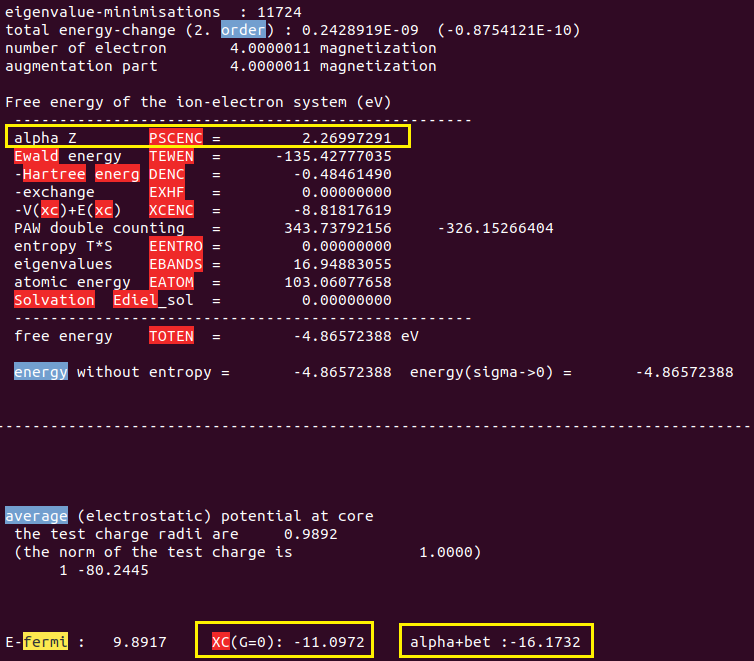
\includegraphics[height=1.85in,width=2.2in,viewport=0 0 600 495,clip]{Figures/VASP_Total_ENE.png}
\caption{\tiny \textrm{The Total-E calculated by VASP.}}%(与文献\cite{EPJB33-47_2003}图1对比)
\label{TOTEN_VASP}
\end{figure}
}

\subsection{模守恒赝势与超软赝势(续)}
\frame
{
	\frametitle{赝势去屏蔽与非局域化}
	第一原理赝势建立了赝波函数与对应赝势的一一对应关系,但该赝势包含了电子屏蔽(原子、离子环境)信息,去屏蔽后的赝势对环境依赖更低,“可移植性”更好
	$$V_{\mathrm{ion},l}^{\mathrm{PP}}(r)=V_{\mathrm{src},l}^{\mathrm{PP}}(r)-V_{\mathrm{H},l}^{\mathrm{PP}}(r)-V_{XC,l}^{\mathrm{PP}}(r)$$
	去屏蔽过程中,特别需要注意$V_{XC,l}^{\mathrm{PP}}(r)$的处理
	$$V_{XC}^{\mathrm{PP}}(r)=V_{XC}^{\mathrm{PP}}([n^{\mathrm{PP}}],r)+\big[V_{XC,l}^{\mathrm{PP}}([n^{\mathrm{PP}}+n^{core}],r)-V_{XC}^{\mathrm{PP}}([n^{\mathrm{PP}}],r)\big]$$
	{\fontsize{7.2pt}{5.2pt}\selectfont{如果定义辅助函数}}
	$$\chi_{lm}^{\mathrm{PP}}(\vec r)=\bigg\{\varepsilon_l-\bigg[-\dfrac12\nabla^2+V_{\mathrm{local}}^{\mathrm{PP}}(\vec r)\bigg]\bigg\}\psi_{lm}^{\mathrm{PP}}(\vec r)$$
	{\fontsize{7.2pt}{5.2pt}\selectfont{赝势可以分解为局域部分与非局域部分之和称为可分离赝势(也称\textrm{factroided pseudo-potential})}}
	$$V_{NL}^{\mathrm{PP}}(r)=V_{\mathrm{local}}^{\mathrm{PP}}(r)+\sum_{lm}\dfrac{|\chi_{lm}^{\mathrm{PP}}\rangle\langle\chi_{lm}^{\mathrm{PP}}|}{\langle\chi_{lm}^{\mathrm{PP}}|\psi_{lm}^{\mathrm{PP}}\rangle}=V_{\mathrm{local}}^{\mathrm{PP}}(r)+\sum_{lm}\dfrac{|\psi_{lm}^{\mathrm{PP}}\delta V_l\rangle\langle\delta V_l\psi_{lm}^{\mathrm{PP}}|}{\langle\psi_{lm}^{\mathrm{PP}}|\delta V_l|\psi_{lm}^{\mathrm{PP}}\rangle}$$
}

\frame
{
\frametitle{超软赝势}
\begin{itemize}
\setlength{\itemsep}{5pt}
	\item 赝势构造的模守恒条件
%		\begin{displaymath}
%			\int_0^{r_c}\mathrm{d}\vec r\varphi^{\ast PS}(\vec r)\varphi^{PS}(\vec r)=\int_0^{r_c}\mathrm{d}\vec r\varphi^{\ast}(\vec r)\varphi(\vec r)
%		\end{displaymath}
	很好地解决了赝势可移植性问题,但对$1s$、$2p$、$3d$等轨道,模守恒方案构造的赝势过于“硬”,所需平面波基组依然非常大
	\item 超软\textrm{(Ultra-soft)}赝势,解除模守恒条件,实现对第一、第二周期元素的高效计算
\end{itemize}
\begin{figure}[h!]
\vspace*{-0.10in}
\centering
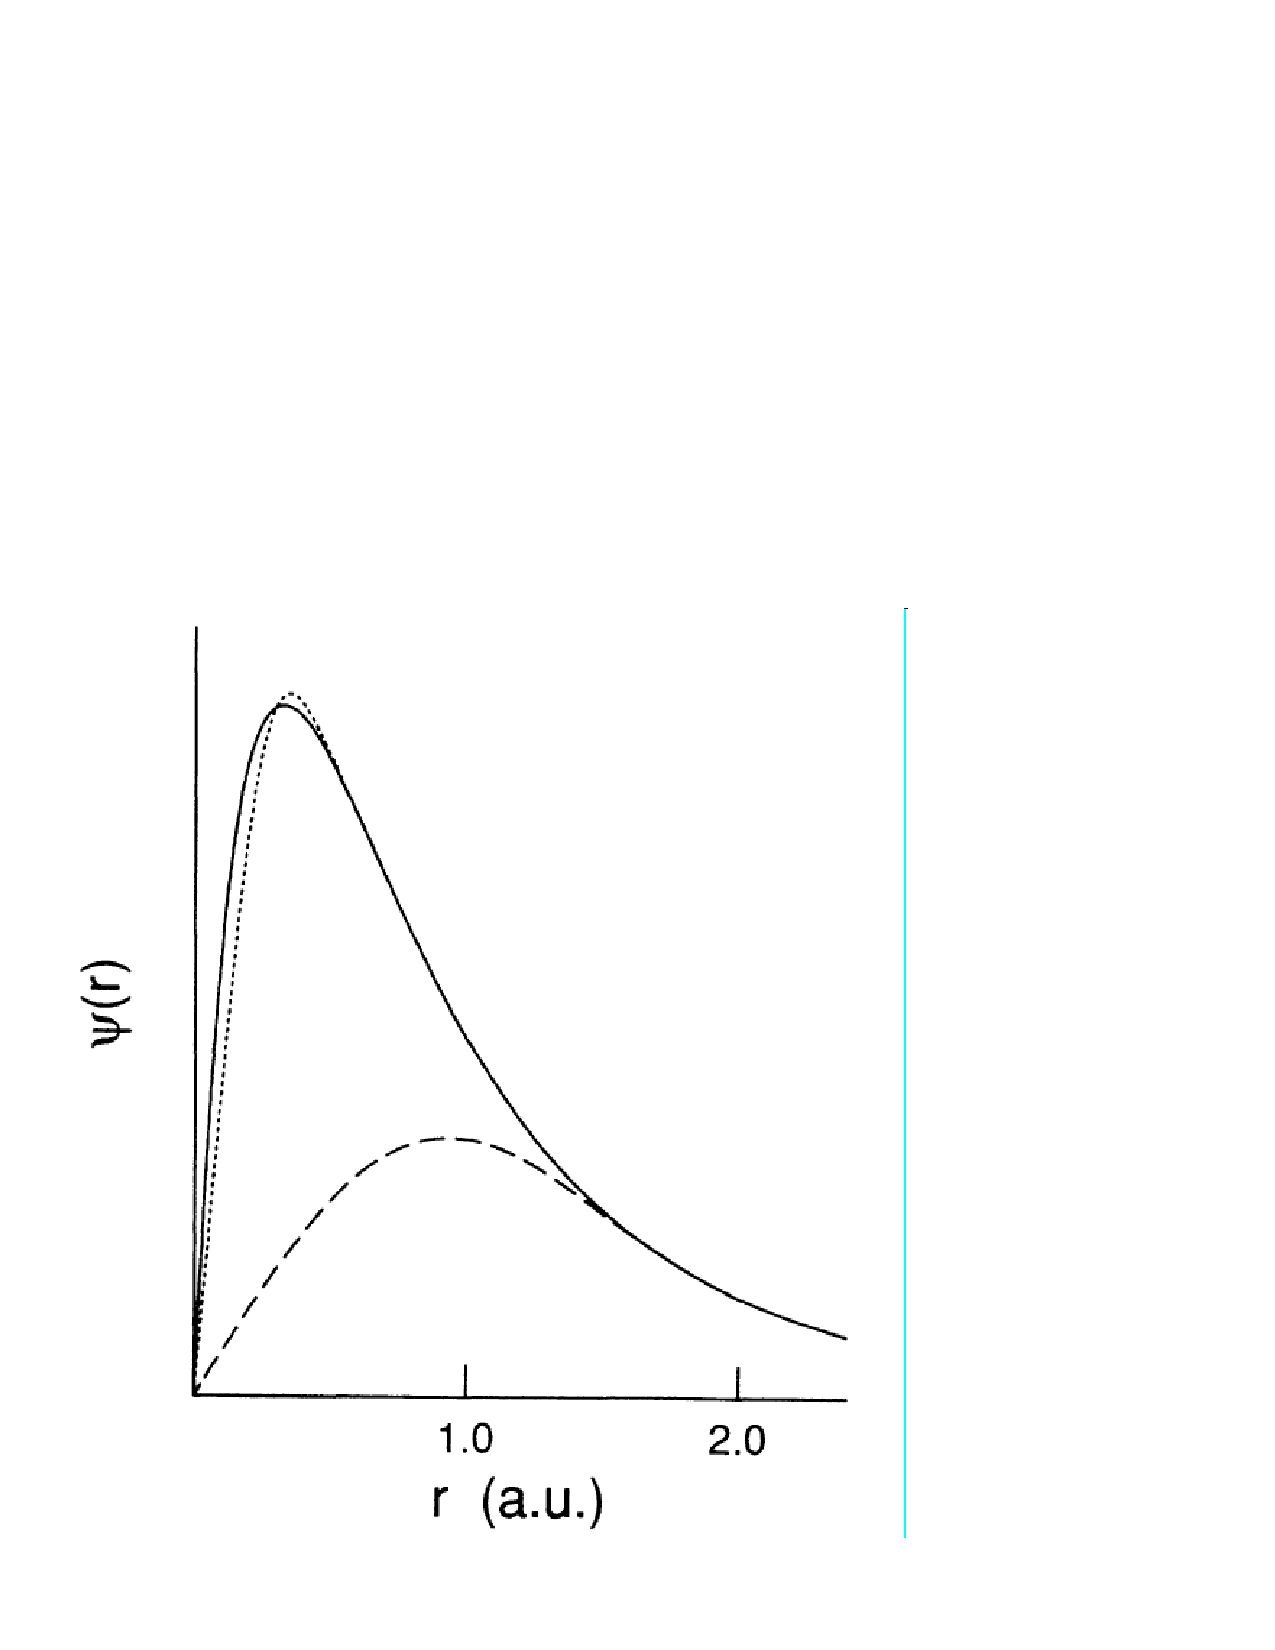
\includegraphics[height=1.35in,width=1.40in,viewport=30 55 415 500,clip]{Figures/Norm-US-wave.pdf}
\caption{\tiny \textrm{Oxygen 2} \textit{p} \textrm{radical wave function (solid), NC-pseudo-wave (dottde) and US-pseudo-wave (dashed).}}%(与文献\cite{EPJB33-47_2003}图1对比)
\label{Norm-US-wave}
\end{figure}
}

\frame
{
	\frametitle{从模守恒赝势到超软赝势}
	为提高模守恒赝势的可移植性\footnote{\tiny{换言之,提升赝波函数能适应的能量变分空间}},\textrm{Vanderbilt}和\textrm{Bl\"ochl}分别建议:\\
	在构造可分离赝势时,\textcolor{blue}{引入额外的参考能量$\varepsilon_l$,并要求对每个角动量量子数$l$,所有能量参数$\varepsilon_l$构造的赝波函数$\phi_i^{\mathrm{ps}}$及其辅助函数$\chi_i$都满足
	\begin{displaymath}
		|\chi_i\rangle=-(\mathbf{T}+V_{\mathrm{loc}}-\varepsilon)|\phi_i^{\mathrm{ps}}\rangle
	\end{displaymath}}
	{\fontsize{7.2pt}{5.2pt}\selectfont{这里$i$表示量子数$l$,$m$和能量参数$\varepsilon$,即$i=(lm,\varepsilon)$}}
	\vskip 5pt
	由此出发,可构造出一组与赝波函数$\phi_i^{\mathrm{ps}}$垂直的函数$\beta_i$:~
{\fontsize{7.2pt}{5.2pt}\selectfont{
	\begin{itemize}
		\item 构造矩阵$\mathbf{B}$,其矩阵元$B_{ij}$满足
			\begin{displaymath}
				B_{ij}= \langle\phi_j^{\mathrm{ps}}|\chi_i\rangle
			\end{displaymath}
		\item 由矩阵$\mathbf{B}$和$\chi$得到函数$\beta_i$
			\begin{displaymath}
				|\beta_i\rangle=\sum_j(\mathbf{B}^{-1})_{ij}|\chi_j\rangle
			\end{displaymath}
		\item 由此得到的$\beta$与赝波函数$\phi_i^{\mathrm{ps}}$满足正交条件
	\begin{displaymath}
		\langle\beta_i|\phi_j^{\mathrm{ps}}\rangle=\delta_{ij}
	\end{displaymath}
	\end{itemize}}}
}

\frame
{
	\frametitle{从模守恒赝势到超软赝势}
	因此可分离赝势的非局域部分表示为
	\textcolor{blue}{\begin{displaymath}
		V_{\mathrm{NL}}=\sum_i|\chi_i\rangle\langle\beta_i|=\sum_{ij}B_{ij}|\beta_j\rangle\langle\beta_i|
	\end{displaymath}}
	{\fontsize{7.2pt}{5.2pt}\selectfont{不难看出,如果赝波函数满足广义模守恒条件
	\begin{displaymath}
		Q_{ij}=\langle\phi_j^{\mathrm{AE}}|\phi_i^{\mathrm{AE}}\rangle-\langle\phi_j^{\mathrm{PS}}|\phi_i^{\mathrm{PS}}\rangle = 0
	\end{displaymath}
	亦即
	\begin{displaymath}
		Q_{l\varepsilon,l\varepsilon^{\prime}}=\int_0^{R_c}\bigg(\phi_{l\varepsilon}^{\mathrm{AE}}(r)\phi_{l\epsilon^{\prime}}^{\mathrm{AE}}(r)-\phi_{l\varepsilon}^{\mathrm{PS}}(r)\phi_{l\varepsilon^{\prime}}^{\mathrm{PS}}(r)\bigg)\mathrm{d}r=0
	\end{displaymath}
	将大大提高赝势的可移植性。
	\vskip 5pt
	但实际上,广义模守恒条件看似简单,当能量参数$\varepsilon\neq\varepsilon^{\prime}$,要满足这个条件
	$$Q_{l\varepsilon,l\varepsilon^{\prime}}=0$$
	并非易事;~而一旦模守恒条件被破坏,矩阵$\mathbf{B}$(相应地,赝势的非局域部分$V_{\mathrm{NL}}$)就是非\textrm{Hermitian}}}
}

\frame
{
\frametitle{超软赝势的构造}
\textrm{Vanderbilt}建议构造赝波函数时放弃模守恒约束条件,只要求价电子赝波函数与真实电子波函数的径向部分在截断半径$r_{c,l}$外相同,由此得到的赝势显然非\textrm{Hermitian},但是通过构造\\\textcolor{blue}{\textrm{Hermitian}重叠算符}
\begin{displaymath}
	\mathbf{S}=\mathbf{1}+\sum_{i,j}Q_{ij}|\beta_j\rangle\langle\beta_i|
\end{displaymath}
以及\textcolor{blue}{\textrm{Hermitian}赝势算符}
\begin{displaymath}
	\tilde V^{\mathrm{NL}}=\sum_{i,j}\mathbf{D}_{i,j}|\beta_j\rangle\langle\beta_i|
\end{displaymath}
这里\textcolor{blue}{
\begin{displaymath}
	\mathbf{D}_{ij}=B_{ij}+\varepsilon_iQ_{ij}
\end{displaymath}}
模守恒约束下的标准本征值方程将变成广义本征值方程
\begin{displaymath}
	(T+V_{\mathrm{loc}}+\tilde V^{\mathrm{NL}}-\varepsilon\mathbf{S})|\phi\rangle=0
\end{displaymath}
}

\frame
{
\frametitle{超软赝势的特点}
\textrm{Vanderbilt}的超软赝势构造方案最大的优点是
\begin{itemize}
	\item \textcolor{purple}{解除模守恒约束}:~有助于增加赝波函数的截断半径,系统提高赝势的柔软程度
	\item \textcolor{purple}{引入多个参考能量$\varepsilon_l$}:~使得模守恒条件下只在特定参考能量$\varepsilon$处成立的对数导数连续条件,扩展到参考能量$\varepsilon_l$区间范围内,这大大提高了赝势的适用范围(可移植性)
\end{itemize}

相应的,超软赝势计算中,电子密度表达形式为
\begin{displaymath}
	n(r)=\sum_nf_n|\phi_n(r)|^2+\sum_{n,ij}f_n\langle\phi_n|\beta_j\rangle\langle\beta_i|\phi_n\rangle Q_{ij}(r)
\end{displaymath}
这里补偿电荷$Q_{ij}(r)$定义为
\begin{displaymath}
	Q_{ij}(r)=\phi_i^{\mathrm{AE}}(r)\phi_j^{\mathrm{AE}}(r)^{\ast}-\phi_i^{\mathrm{US}}(r)\phi_j^{\mathrm{US}}(r)^{\ast}
\end{displaymath}
}

\frame
{
\frametitle{补偿电荷与多极矩}
根据电动力学定理:\\\textcolor{blue}{如果球\textrm{S}内的电荷密度分布$\rho(\vec r)$,在球外某点$\vec r$产生的势是由电荷密度的多极矩确定}:
\begin{figure}[h!]
\vspace*{-15pt}
\centering
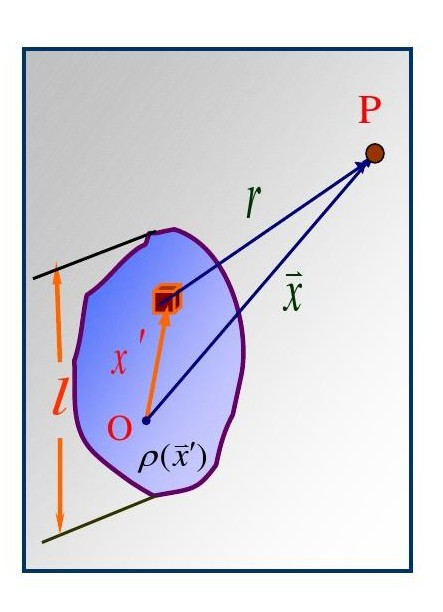
\includegraphics[height=1.25in,width=1.32in,viewport=1 22 507 575,clip]{Figures/potential_multipole.jpg}
%\caption{\tiny \textrm{From Muffin-tin Potential to Full Potential}}%(与文献\cite{EPJB33-47_2003}图1对比)
\label{Potential-multipole}
\end{figure}
\begin{displaymath}
	V(\vec r)=\sum_{l=0}^{\infty}\sum_{m=-l}^{l}\dfrac{4\pi}{2l+1}q_{lm}\dfrac{Y_{lm}(\hat{\vec r})}{r^{l+1}}
\end{displaymath}
其中多极矩$q_{lm}$由下式计算
\begin{displaymath}
	q_{lm}=\int_SY_{lm}^{\ast}(\hat{\vec r})r^l\rho(\vec r)\mathrm{d}^3r
\end{displaymath}
}

\frame
{
	\frametitle{超软赝势总能量计算}
	去除价电子屏蔽效应的贡献后,可得最终超软赝势的总能量表达式
	\begin{displaymath}
		\begin{aligned}
			E_{\mathrm{total}}=&\sum_j^{\mathrm{occ}}\langle\phi_{lmj}|\bigg[-\dfrac12\nabla^2+V_{\mathrm{local}}^{\mathrm{ion}}+\sum_{s,s^{\prime}}\mathbf{D}_{s,s^{\prime}}^{\mathrm{ion}}|\beta_s\rangle\langle\beta_{s^{\prime}}|\bigg]|\phi_{lmj}\rangle\\
			&+E_{H}[n_v]+E_{N-N}+E_{XC}[n_v]
		\end{aligned}
	\end{displaymath}
	{\fontsize{7.2pt}{5.2pt}\selectfont{其中$n_v(r)=\sum\limits_j^{\mathrm{occ}}\phi_{lmj}^{\ast}(r)\phi_{lmj}(r)+\sum\limits_{s,s^{\prime}}\sum\limits_j^{\mathrm{occ}}\langle\phi_{lmj}|\beta_{s^{\prime}}\rangle\langle\beta_s|\phi_{lmj}\rangle Q_{s,s^{\prime}}(r)$
	$$V_{\mathrm{local}}^{\mathrm{ion}}=V_{\mathrm{local}}-V_{\mathrm H}-V_{XC}$$
	$$\mathbf{D}_{s,s^{\prime}}^{\mathrm{ion}}=\mathbf{D}_{s,s^{\prime}}-\int\mathrm{d}\vec r\big[V_{\mathrm{H}}(\vec r)+V_{XC}(\vec r)\big]Q_{s,s^{\prime}}(r)$$}}
	由此可得超软赝势的广义本征值方程
	$$\bigg[-\dfrac12\nabla^2+V_{\mathrm{local}}+\tilde V_{NL}^{\mathrm{US}}-\varepsilon_i\bigg(\mathbf{1}+\sum_{s,s^{\prime}}Q_{s,s^{\prime}}|\beta_s\rangle\langle\beta_{s^{\prime}}|\bigg)\bigg]|\phi_{lmi}\rangle=0$$
}

\frame
{
	\frametitle{赝势方法发展概要}
\begin{figure}[h!]
\centering
\vspace*{-0.25in}
%\hspace*{-0.80in}
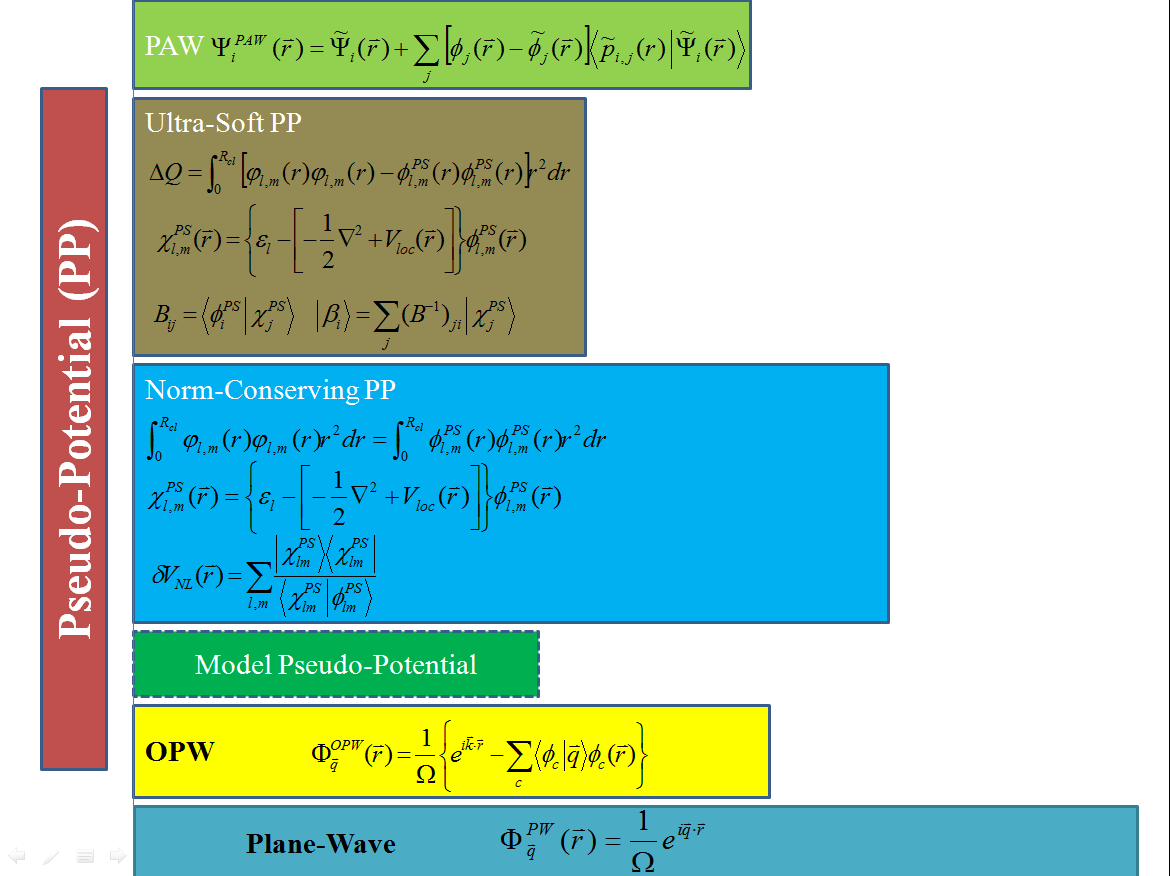
\includegraphics[height=2.80in,width=4.10in,viewport=0 0 1190 875,clip]{Figures/Pseudo_Potential.png}
%\caption{\tiny \textrm{Pseudopotential for metallic sodium, based on the empty core model and screened by the Thomas-Fermi dielectric function.}}%(与文献\cite{EPJB33-47_2003}图1对比)
\label{Pseudo_Poential}
\end{figure}
}

